\section{Angriffe}
Im Rahmen dieser Ausarbeitung wollen wir uns auf die Ermittlung des \textit{Pre-shared Keys} (\textit{PSK}) als Angriffsziel und auf den Angriffsvektor des Brechens mitgeschnitttener Handshakes durch Exploration des Schlüsselraumes (Bruteforce) beschränken.

Tatsächlich gibt es nach dem bekannten Stand der Forschung keine Schwachstellen im Protokoll von WPA2-PSK, die es einem, nicht der Nutzergruppe angehörenden, Angreifer ermöglichen würden, die Kommunikation zu entschlüsseln. Es gibt bspw. eine Schwachstelle (\enquote{Hole 196}), die die Ermittlung des PTKs anderer Teilnehmer ermöglicht -- allerdings muss dem Angreifer hierfür der PSK bekannt sein, was die praktische Relevanz des Angriffes drastisch reduziert.

Aufgrund der Aufmerksamkeit, der sich dieses Thema unter Netzwerkexperten und Kryptologen in der Vergangenheit erfreute, ist nicht damit zu rechnen, dass in dem Verfahren noch grundlegende Schwachstellen gefunden werden. 

Da die Sicherheit eines solchen Verfahrens jedoch von mindestens drei Dingen abhängt -- der Sicherheit des Protokolls sowie der kryptografischen Primitiven, der fehlerfreien Implementierung und auch der Wahl eines guten Geheimnisses -- reicht dies allein nicht aus. 
So liegt die Wahl des Geheimnisses (in diesem Fall des Netzwerkschlüssels) meist in der Hand des nicht zwingend sachverständigen Endnutzers. 
So kann ein schlecht gewähltes Passwort oftmals durch einen durchdachten Wörterbuchangriff in realistischer Zeit gebrochen werden, ohne das Protokoll als solches angreifen zu müssen.

Die im Standard beschriebenen Anforderungen an einen PSK legen lediglich eine Länge von 8 Zeichen fest. \cite{zviran1999password} zufolge wählen Nutzer im Mittel lediglich 6 Zeichen lange Passwörter und greifen darauf in 8 von 10 Fällen ausschließlich auf Buchstaben zurück. Nur 13,7 \% der in dieser Studie analysierten Passwörter waren alphanumerisch. Auch wenn man davon ausgeht, dass Privatanwender für ihr WLAN womöglich ein vergleichsweise langes Passwort wählen, da sie es nicht täglich eingeben müssen -- so werden sie vermutlich weiterhin auf Wörter oder gängige Wort-Zahl-Kombinationen zurückgreifen, um es bspw. einfach an Gäste weitergeben zu können.
Auch finden sich immer wieder Berichte über schlechte Standardpasswörter \cite{stanched2015defaultpasswords}, mit denen die Geräte seitens des Herstellers oder ISPs ausgeliefert werden. Die Hoffnung, auf ein schwaches Passwort zu stoßen ist daher keinesfalls unbegründet -- und wie später dargelegt werden soll, hängt die gesamte Sicherheit je nach Angriff vom am schwächsten gesicherten Netzwerk ab, dass dem Gerät bekannt ist.\\

Eine weitere Spielweise sind Social-Engineering-Angriffe, die auf Unwissenheit, Unaufmerksamkeit und Leichtgläubigkeit der Nutzer setzen. 
Durch die nachfolgend beschriebene \enquote{Auskunftsfreudigkeit} der meisten Endgeräte hinsichtlich ihrer bekannten Netzwerke ergeben sich für Tools dieser Kategorie Möglichkeiten ihre Angriffe plausibel und für die meisten Nutzer authentisch wirkend durchzuführen.
So strahlt zum Beispiel das Tool \textit{wifiphisher} über einen geeigneten Netzwerk-Adapter ein offenes Netzwerk mit beliebiger SSID aus und präsentiert verbundenen Nutzern je nach System verschiedene, teils täuschend echt aussehende Dialoge zur Eingabe des Netzwerkschlüssels. 
Um einen Nutzer in das eigene Netzwerk zu bringen nutzt das Tool den später beschriebenen Deauth-Angriff. 

\textit{Fluxion} prüft die vom Benutzer getätigten Eingaben zusätzlich gegen einen mitgeschnittenen Handshake ab und kann sich so dem Benutzer gegenüber authentisch Verhalten und Falscheingaben erkennen. 
Dieser und weitere Angriffe, wie sie beispielsweise in~\cite{caneill2010attacks} beschrieben sind, sollen in dieser Ausarbeitung jedoch nicht weiter betrachtet werden, da ihr Ansatz ein grundlegend anderer ist.\\

\subsection{Erfassen eines WPA2-Handshakes}
Bei Bruteforce-Angriffen unterteilt sich die Ermittlung des Netzwerkschlüssels (PSK) in zwei elementare Schritte: 
\begin{enumerate}
	\item Die Erfassung eines WPA2-PSK-Handshakes während der Authentifizierungsphase zwischen Client und AP
	\item Die nachgelagerte Suche nach einem Schlüssel, der zu einem gleichen \textit{Message Integrity Code} führt
\end{enumerate}
Die vermutlich subtilste Methode zur Erlangung eines Handshakes, die dem Angreifer zur Verfügung steht, ist die passive Überwachung des Netzwerkverkehrs.
Dafür muss er lediglich abwarten, bis sich ein Client gegenüber einem AP im gewünschten Netzwerk authentifiziert. 
Abhängig von der Netzwerkinfrastruktur und des Nutzungsverhaltens des Clients kann dies jedoch viel Zeit in Anspruch nehmen.
Da dies für einen gezielten Angriff nicht zielführend erscheint werden nachfolgend zwei Angriffe beschrieben, die durch aktives Eingreifen in den Netzwerkverkehr die Authentifizierung des Clients forcieren.

\subsubsection{Deauth-Angriff}\label{subs:deauth-attack}
Wie in Kapitel~\ref{sec:grundlagen} bereits beschrieben definiert IEEE 802.11 neben Daten- und Kontroll-Frames unter anderem auch Management-Frames, die der Verwaltung des Netzwerkes dienen und weder verschlüsselt noch anderweitig authentifiziert auf dem exponierten Übertragungsmedium versendet werden.

Dies hat zur Folge, dass ein Angreifer Management-Frames erzeugen und im Netzwerk unter einem gefälschten Absender an beliebige Teilnehmer verteilen kann.
So auch Deauthentication-Frames, mit denen ein Access-Point die erneute Authentifizierung eines Clients vor einer weiteren Nutzung erzwingen kann. Die Idee ist nun sehr simpel: Der Angreifer kennt sein Opfer, gaukelt diesem durch gefälschte Deauthentication-Frames die Deauthentifizierung durch den AP vor um anschließend den provozierten Handshake mitschneiden zu können.
Die Felder des entsprechenden Deauthentication-Frame werden dabei wie folgt gesetzt:
\begin{itemize}
	\item als Zieladresse (DA) die MAC-Adresse des Clients
	\item als Quelladresse (SA) die MAC-Adresse des Access-Points
	\item als BSSID die MAC-Adresse des AP mit dem der Client kommuniziert
	\item ein beliebiger Reason-Code, bspw. \enquote{1} für \enquote{Unspecified Reason} \cite[S. 442]{ieee802.11}
\end{itemize}
Abbildung~\ref{fig:deauth-attack} zeigt ein solches Deauthentication-Frame sowie die vom Angreifer zu modifizierenden Felder.

\begin{figure}[ht]
	\centering
	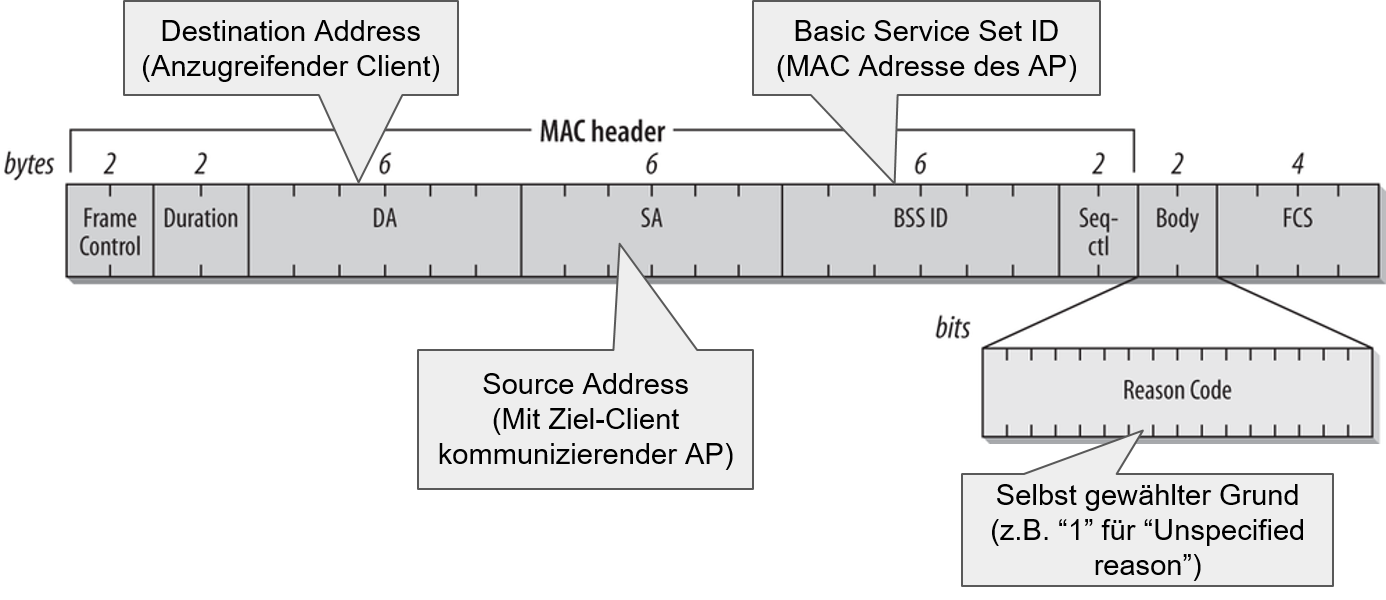
\includegraphics[width=0.7\textwidth]{graphics/deauth-attack}
	\caption[Deauthentication-Frame]{Abbildung eines Deauthentication-Frames~\cite{deauthframe}.}
	\label{fig:deauth-attack}
\end{figure}

Gemäß Spezifikation entspricht in Netzwerken, welche eine Authentifizierung erzwingen, eine Deauthentifizierung einer Disassozierung (durch ein Disassociation-Frame herbeigeführte Verbindungsaufhebung)\footcite[S. 74, S. 442]{ieee802.11}. In einen einem Versuch gegen ein mit \textit{macOS 10.12.4} betriebenes Gerät konnten wir zeigen, dass -- auch wenn der Name es nicht suggeriert -- die Verwendung von Disassociation-Frames für diesen Angriff ebenfalls geeignet ist.

\paragraph{Durchführung}
Zur Durchführung des Deauth-Angriffs müssen zwei Voraussetzungen erfüllt sein: 
\begin{itemize}
	\item der Client ist mit einem AP des Zielnetzwerks verbunden; dieses operiert nach IEEE 802.11
	\item der Angreifer befindet sich in Reichweite zu Client und dessen AP
\end{itemize}

Wie für alle in dieser Arbeit beschriebenen, praktischen Angriffe und Evaluationen wird ein WLAN-Chipset benötigt, dessen Treiber kompatibel mit der \texttt{aircrack-ng}-Suite sind. 
Zunächst versetzt der Angreifer sein Netzwerkinterface (z.B. \texttt{wlan0}) in den \enquote{Monitor-Mode}\footnote{Im Monitor-Modus verarbeitet das Interface alle eingehenden Pakete, nicht nur solche, die an die MAC-Adresse des Empfängers gerichtet sind oder als Broadcast verteilt werden.} und beendet interferierende Hintergrundprozesse:

\begin{Verbatim}
	airmon-ng check kill
	airmon-ng start <Interface im Monitor-Mode>
\end{Verbatim}

Dies ermöglicht das Überwachen des Netzwerkverkehrs und das aussenden eigens erstellter Frames.
Um potentielle Handshakes und andere Pakete aufzuzeichnen verwendet der Angreifer \texttt{airodump-ng}:
\begin{Verbatim}
	airodump-ng -c <Ch> --bssid <AP-MAC> -w <Dateiname> <Interface>
\end{Verbatim}
Ist der Channel nicht bekannt, so kann \texttt{airodump-ng} auch \enquote{Channel-Hopping} betreiben. 
Dies führt in der Praxis jedoch verständlicherweise zu Paketverlusten, weshalb es sich empfiehlt, den Channel vorher in Erfahrung zu bringen. Das Flag \texttt{--bssid} ist optional und dient als Filter. Es verhindert, dass Pakete von anderen APs aufgezeichnet werden und kann somit die nachträgliche Analyse erleichtern und die Datenmenge kleiner halten. Der Einsatz empfiehlt sich womöglich auch aus rechtlicher Perspektive.

Sind die MAC-Adressen des Clients und des AP bekannt startet der Angreifer mit Hilfe von \texttt{aireplay-ng} den Deauth-Angriff: 
\begin{Verbatim}
	aireplay-ng -0 <Anzahl> -a <AP-MAC> -c <Client-MAC> <Interface>
\end{Verbatim}
Das Flag \texttt{-0} kennzeichnet dabei den Deauth-Angriff.
Via \texttt{<Anzahl>} kann spezifiziert werden, wie viele Deauthentication-Frames an das Ziel gesendet werden.
In unseren Versuchen hat sich gezeigt, dass es meistens mehrerer Deauthentication-Pakete bedurfte, um den Client tatsächlich zu einem kurzzeitigen Verlassen des Netzwerkes zu bewegen. Die Wahl der Anzahl hat sich hierbei als Gratwanderung herausgestellt: werden zu wenig Pakete versendet führt der Client keine erneute Authentifizierung durch -- werden jedoch zu viele Pakete versendet, so konnten wir beobachten wie das Endgerät sich mit einem eigentlich niedriger priorisiertem Netzwerk verbunden hat, da ihm einer erneuter Verbindungsaufbau anscheinend nicht möglich erschien. Ein Wert von 20 hat sich in unseren Versuchen als zielführend erwiesen.
Ein Nachteil dieses Ansatzes ist, dass \texttt{aireplay-ng} mit dem Aussenden der Deauthentication-Frames wartet bis es einen Beacon-Frame des Access-Points erhalten hat -- eine technische Notwendigkeit hierfür besteht unserer Ansicht nach nicht.
Alternativ kann die Deauthentifikation mit wenigen Zeilen Python-Code unter Verwendung der Bibliothek \texttt{Scapy} durchgeführt erden.

\begin{minted}[breakbytoken,breaklines]{python}
	import scapy.all as scapy
	# Construct a deauth packet, subtype 12 
	# is the 802.11 code for a deauthentication-frame
	# bssid is equivalent to the MAC of the AP
	p = scapy.RadioTap() / scapy.Dot11(type=0, subtype=12, addr1=clientMac, addr2=bssid, addr3=bssid) / scapy.Dot11Deauth(reason=1)
	scapy.send(p)
\end{minted}

Nach dem Angriff wird die eingangs gestartete Netzwerkaufzeichnung mit \texttt{airodump-ng} gestoppt, um den Dump mithilfe eines geeigneten Tools, zum Beispiel \texttt{Pyrit}, zu analysieren. Dieser Schritt ist optional, die schnelle Verifikation womöglich jedoch hilfreich\footnote{Wurde die MAC-Adresse des Access-Points nicht beim Aufzeichnen des Verkehrs spezifiziert sollte sie nun mit dem Flag \texttt{-b} festgelegt werden.
Andernfalls wird \texttt{Pyrit} für eventuell weitere aufgezeichnete Handshakes von anderen Netzwerken positiv antworten.}: 
\begin{Verbatim}
	pyrit -r <Dump-Name> -b <AP-MAC> analyze
\end{Verbatim}
Ein im Rahmen der Arbeit geschriebenes Python-Skript, welches unter Anderem die oben beschriebenen Schritte automatisiert, findet sich auf \textit{GitHub}\footnote{\href{https://github.com/kastel-wpa2/deauth-tool/blob/master/deauth_jammer.py}{https://github.com/kastel-wpa2/deauth-tool/blob/master/deauth\_jammer.py}}. Ein ebenfalls für diese Arbeit gebautes Tool nutzt unter anderem dieses Skript, um Deauth-Angriffe und das vorangehende Scannen des Netzwerkverkehrs komfortabel über eine Weboberfläche zu ermöglichen\footnote{\href{https://github.com/kastel-wpa2/deauth-tool/blob/master/tool.py}{https://github.com/kastel-wpa2/deauth-tool/blob/master/tool.py}}.
Der Versuch des Brechens des erlangten Handshakes wird in Unterkapitel~\ref{subs:cracking} erläutert.

\subsubsection{\enquote{Evil-Twin}-Angriff}\label{subs:evil-twin-attack}
Ein Nachteil des Deauth-Angriffs ist, dass sowohl Client als auch AP in Reichweite des Angreifers sein müssen (\enquote{on-site}), um den Handshake zwischen beiden abfangen zu können. Der Evil-Twin-Angriff als \enquote{off-site}-Attacke hebt diese Beschränkung auf. Die Idee hierbei ist, einen AP zu imitieren, der einem dem Client bekannten Netzwerk angehört. Auf diese Weise wird der Client zur Durchführung eines Handshakes verleitet, auch wenn das eigentliche Netzwerk nicht in Reichweite ist. 
%Je nach Quelle überlappt der Evil-Twin Angriff mit dem des \textit{Rogue-Access-Points} -- teilweise werden die Begriffe auch synonym verwendet.\\
%TODO: würde ich raus nehmen... klingt blöd und die einzigen die das hier lesen werden wissen was ein evil twin ist
Betrachtet man den Ablauf des Handshakes (siehe Unterkapitel~\ref{subs:handshake}), so stellt man fest, dass die für einen Bruteforce-Angriff wichtigen Elemente keines vollständigen Handshakes bedürfen. Benötigt werden lediglich folgende Informationen:
\begin{itemize}
	\item SSID des Netzwerkes 
	\item MAC-Adressen der beiden Kommunikationspartner
	\item \textit{ANonce} aus Schritt 1
	\item \textit{SNonce} inklusive \textit{MIC} aus Schritt 2
\end{itemize}
Die Parameter, die vom AP übermittelt werden, unterliegen keinerlei Schutz und werden nicht auf Authentizität geprüft.
Der Angreifer kann demnach die ANonce und MAC-Adresse beliebig wählen und den Handshake bis zu Schritt zwei durchführen.
Um die übrigen Parameter zu erhalten (SNonce inklusive MIC) muss der Angreifer dem Client ein authentisches, ihm bekanntes Netzwerk vortäuschen -- den \enquote{Evil-Twin}. In der Praxis ist meist eine bekannte SSID und Sicherheitskonfiguration ausreichend. Letztere entspricht einer der folgenden Möglichkeiten (Unterkonfigurationen nicht betrachtet): Open (kein Schutzverfahren), WEP, WPA-PSK, WPA-Enterprise, WPA2-PSK, WPA2-Enterprise.
Die Anzahl der in der Praxis gängigen Konfigurationen ist sehr begrenzt, der Angreifer kann dementsprechend einfach alle populären Konfigurationen durch einen eigenen, virtuellen AP abdecken. Ist das Zielnetzwerk bekannt (und somit auch die SSID), so ist der Evil-Twin einsatzbereit.

Oft ist jedoch ein konkreter Client Ziel des Angriffs und nicht ein bestimmtes Netzwerk, wenn das Ziel bspw. die Kontrolle von dessen Kommunikation via Man-in-the-Middle-Methoden ist. Prinzipiell sind dem Angreifer die dem Client bekannten Netzwerke verborgen, sofern er nicht gerade aktiv mit diesen kommuniziert.
An dieser Stelle kommen die in Abschnitt~\ref{subs:probes} beschriebenen Probe-Requests in Spiel, die je nach Client kontinuierlich gesendet werden.
Aus diesen kann der Angreifer die SSIDs bekannter Gegenstellen auslesen und gegebenenfalls mehrere APs starten.

Auf diese Art und Weise ist es möglich automatisiert und in kurzer Zeit viele Handshakes für viele verschiedene Netzwerke einzusammeln. Diese dienen dann als Grundlage für einen Angriff in die Breite: Anstelle von komplexen Passwörtern als Kandidaten  für den Bruteforce-Schritt zu wählen, werden nur solche mit einer vergleichsweise hohen Wahrscheinlichkeit verwendet -- jedoch gegen viele Handshakes. Die Annahme dahinter ist, dass wichtige Netzwerke zwar gut gewählte Passwörter verwenden -- die meisten Endgeräte jedoch auch schon mit schlecht geschützten \enquote{Café-WLANs} verbunden waren.

Liegt der Fokus auf der gezielten Kompromittierung eines bestimmten Nutzers, so hängt die Sicherheit der WLAN-Verbindung nun von der Komplexität des schwächsten PSKs ab. Geht es um den Zugriff auf ein bestimmtes Netzwerk, so ist diese Suche nach der \enquote{lowest hanging fruit} nicht zielführend.

\paragraph{Durchführung}
Für den Evil-Twin Angriff bietet die \texttt{aircrack-ng}-Suite zwei mögliche Herangehensweisen, die folgend näher beleuchtet werden sollen.
Zunächst muss, wie beim Deauth-Angriff bereits beschrieben, das Netzwerkinterface in den Monitor-Mode versetzt werden.
Weiß der Angreifer im Vorfeld für welche SSID er den Evil-Twin öffnen möchte, so kann er dafür den folgenden Befehl verwenden:
\begin{Verbatim}
	airbase-ng start --essid <SSID> -Z 4 -F <Dateiname> <Interface>
\end{Verbatim}

Durch das Flag \texttt{-Z 4} wird sich der Evil-Twin als AP eines WPA2-PSK geschützten Netzwerks ausgeben.
Mithilfe von \texttt{-F <Dateiname>} wird der Netzwerkverkehr zwischen dem Evil-Twin und den Clients mitgeschnitten.
Versucht sich ein Client nun mit dem Evil-Twin zu verbinden, so wird der Handshake bis zu Schritt zwei durchgeführt und anschließend abgebrochen.
Dies äußert sich beim Client in Form einer Fehlermeldung wie zum Beispiel: \enquote{Fehler bei der Authentifizierung}. \\

\begin{figure}[ht]
	\centering
	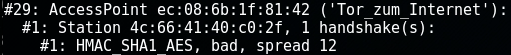
\includegraphics[width=0.7\textwidth]{graphics/pyrit_analyze}
	\caption[Pyrit]{Auch dem mitgeschnittenen Handshake sieht man an, dass es sich nur um einen \enquote{halben Handshake} handelt -- der obenstehende Aufruf von \texttt{pyrit} markiert ihn als \enquote{Bad}, da er nicht erfolgreich bzw. komplett durchgeführt wurde. Für einen Angriff eignet er sich dennoch.}
\end{figure}
\FloatBarrier

Kennt der Angreifer keine seinem Ziel bekannten SSIDs, so kann er das \texttt{-P}-Flag verwenden:
\begin{Verbatim}
	airbase-ng start -P -Z 4 <Interface>
\end{Verbatim}

\texttt{airbase-ng} wird nun auf dem ausgewählten Interface Probe-Requests von Clients auswerten, um automatisch Evil-Twins mit der vom Angreifer spezifizierten Konfiguration zu erzeugen.
Es empfiehlt sich, gleichzeitig einen \texttt{airodump-ng} Prozess zu starten, welcher den Verkehr des Evil-Twins separat aufzeichnet.
Dies hat den Hintergrund, dass die Aufzeichnung von \texttt{airbase-ng} ohne spezifizierte SSID via \texttt{--essid} Flag \texttt{default} als Netzwerknamen verwendet -- anstelle des Wertes aus dem Probe-Request. Dies führt in späteren Schritten zu Problemen, denn ohne gültige SSID werden Handshakes unbrauchbar, da diese in die Berechnung des PMK mit einfließt (und von \texttt{aircrack-ng} automatisch aus dem Dump extrahiert wird).

\subsection{Handshake-Bruteforcing}\label{subs:cracking}
Liegen valide Handshake-Mitschnitte vor, so kann der Angreifer versuchen den PSK offline zu brechen.
Dafür spielt er die Schritte, die Client und AP während des Handshakes durchführen, lokal nach und wählt in jeder Iteration einen neuen Passwortkandidaten.
Die Vorgehensweise entspricht folgendem Algorithmus (siehe auch Abbildung~\ref{fig:wpa2handshake}):
\begin{enumerate}
	\item Berechne $\mathsf{PMK} = \mathsf{PBKDF2}(\mathsf{SSID}, \mathsf{PSK}, 4096, 256)$
	\item Verwende die aufgezeichneten Noncen und berechne damit \\$\mathsf{PTK} = \mathsf{PRF}(\mathsf{Client-MAC},  \mathsf{Access-Point-MAC}, \mathsf{SNonce}, \mathsf{ANonce}, \mathsf{PMK})$
	\item Bilde den $\mathsf{MIC}$ über den $\mathsf{PTK}$-Kandidaten und vergleiche ihn mit dem aufgezeichneten $\mathsf{MIC'}$
	\begin{enumerate}
		\item $\mathsf{MIC} \neq \mathsf{MIC'}$: Neustart von Schritt 1
		\item $\mathsf{MIC} = \mathsf{MIC'}$: Kollision gefunden, Handshake erfolgreich gebrochen
	\end{enumerate}
\end{enumerate}
Der Großteil des Rechenaufwands lässt sich auf das Bilden des PMKs in Schritt 1 durch $4096$ Runden PBKDF2 zurückführen. Ein AP muss diese Rechnung nur einmal durchführen, da sie lediglich von statischen Eingaben abhängt. %Rechenaufwand ist nicht durch die 4096 Runden "immens", sondern durch den großen Passwortraum
Des Weiteren kann nur sehr selten auf vorab generierte PMK-Listen zurückgegriffen werden, da der PMK auch von der SSID des Netzwerkes abhängig ist. Solche Listen existieren, allerdings nur für die häufigsten SSIDs. Als Tool zu ihrer Erzeugung sei hier \texttt{coWPAtty} genannt.\\

Auf Grund des gigantischen zu explorierendes Suchraumes, sind in der Praxis für den Angreifer zufällige Passwörter lediglich bis zu einer gewissen Länge zu brechen. Die Festlegung auf genau Acht alphanumerische Zeichen ergäbe so bspw. 218.340.105.584.896 zu testende Kandidaten. Auf einem \textit{Apple MacBook Pro 13"} (Mid 2014), ausgestattet mit einem \textit{Intel i5} mit 2,8 Ghz, wurden mit \textit{aircrack-ng} ca. 1,8 kHashes/s erreicht. Mit einem GPU-Cluster wie dem \textit{Sagitta Brutalis}\footnote{Bestehend aus acht \textit{Nvidia GTX 1080} und zwei \textit{Intel Xeon E5 2620V3}, Preis circa 18500 \$} lassen sich bspw. ca 3,2 gHashes/s erreichen\cite{sagittabrutalisbenchmark}. Ähnliche Kapazitäten lassen sich bspw. auch bei IaaS-Anbietern wie \textit{Amazon AWS} anmieten. Im Mittel würden für einen erfolgreichen Angriff auf dieses Passwort immer noch ca. 400 Tage benötigt werden.
Erzeugen sich Passwörter jedoch nach gängigem Schema aus Wörtern, Ziffern und häufigen Sonderzeichen, so fällt der Suchraum massiv in sich zusammen. Angenommen, ein Passwort besteht aus einem Wort, das zu den 10.000 häufigsten der hier bekannten Sprache gehört, und zwei Ziffern. Das Passwort mag nun weiterhin eine Länge von acht Zeichen haben, es ergeben sich allerdings nur noch 1 Million Kombinationen -- ein Angriff würde keine Sekunde benötigen.

Dies soll verdeutlichen, dass ein \enquote{blinder} Bruteforce-Angriff ohne jedwede Annahmen bzgl. des Suchraumes in der Praxis nicht erfolgversprechend sind -- eine weitere Besprechung hinsichtlich zielführender Vorannahmen etc. würden den Rahmen dieser Arbeit sprengen.

\paragraph{Durchführung}
Es existieren verschiedenste Tools und Online-Services zum Brechen von WPA2-PSK Handshakes, deren Funktionsweise letztlich immer dieselbe ist.

In dieser Arbeit werden die Beispiele mit \texttt{aircrack-ng} (als Teil der gleichnamigen Suite) gezeigt. Erwähnt seien jedoch noch die Programme \texttt{oclhashcat} bzw. \texttt{cudahashcat}, welche durch den Einsatz der massiven Parallelität moderner GPUs eine deutlich höhere Hashes/Sekunde-Rate ermöglichen sowie \texttt{John The Ripper}, welches auch unter Microsoft Windows arbeitet. Im Gegensatz zu \texttt{aircrack-ng} unterstützen diese eine Vielzahl weiterer Algorithmen neben den für WPA2-PSK benötigten.\\

\texttt{Aircrack-ng} benötigt zum Brechen ein Mitschnitt, der die ersten zwei Schritte des WPA2-PSK Handshakes enthält.
Weiterhin ist eine Passwortliste erforderlich die PSK Kandidaten enthält, welche \texttt{aircrack-ng} für den aufgezeichneten Handshake prüfen soll. Alternativ können diese über die Standardeingabe hineingereicht werden.
\begin{Verbatim}
	aircrack-ng -w <Passwortliste> -b <AP-MAC> <Capture> # mit Liste
	crunch ... | aircrack-ng -w - -b <AP-MAC> <Capture> # über stdin
\end{Verbatim}
\texttt{Crunch} ist hierbei ein Tool zur Generierung von Passwortkandidaten auf Basis bestimmter Vorgaben.
Sofern während der Aufzeichnung sichergestellt wurde, dass ausschließlich Verkehr des gewünschten Funkzelle aufgezeichnet wurde, so kann das Flag \texttt{-b} verworfen werden.

\begin{figure}[ht]
	\centering
	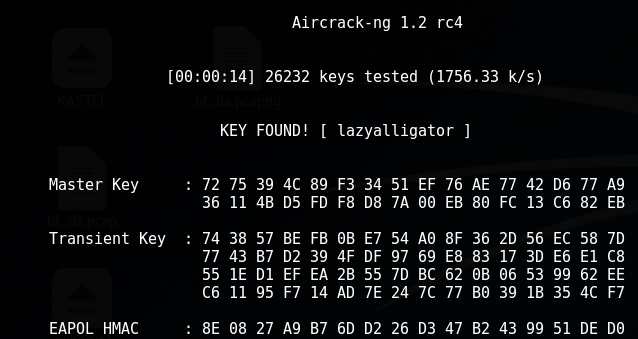
\includegraphics[width=0.7\textwidth]{graphics/aircrack_success}
	\caption[Aircrack-ng]{\texttt{aircrack-ng} hat den gültigen PSK gefunden}
\end{figure}

\FloatBarrier